\begin{figure}[h!]
	\centering
	\subfloat[Full]{
		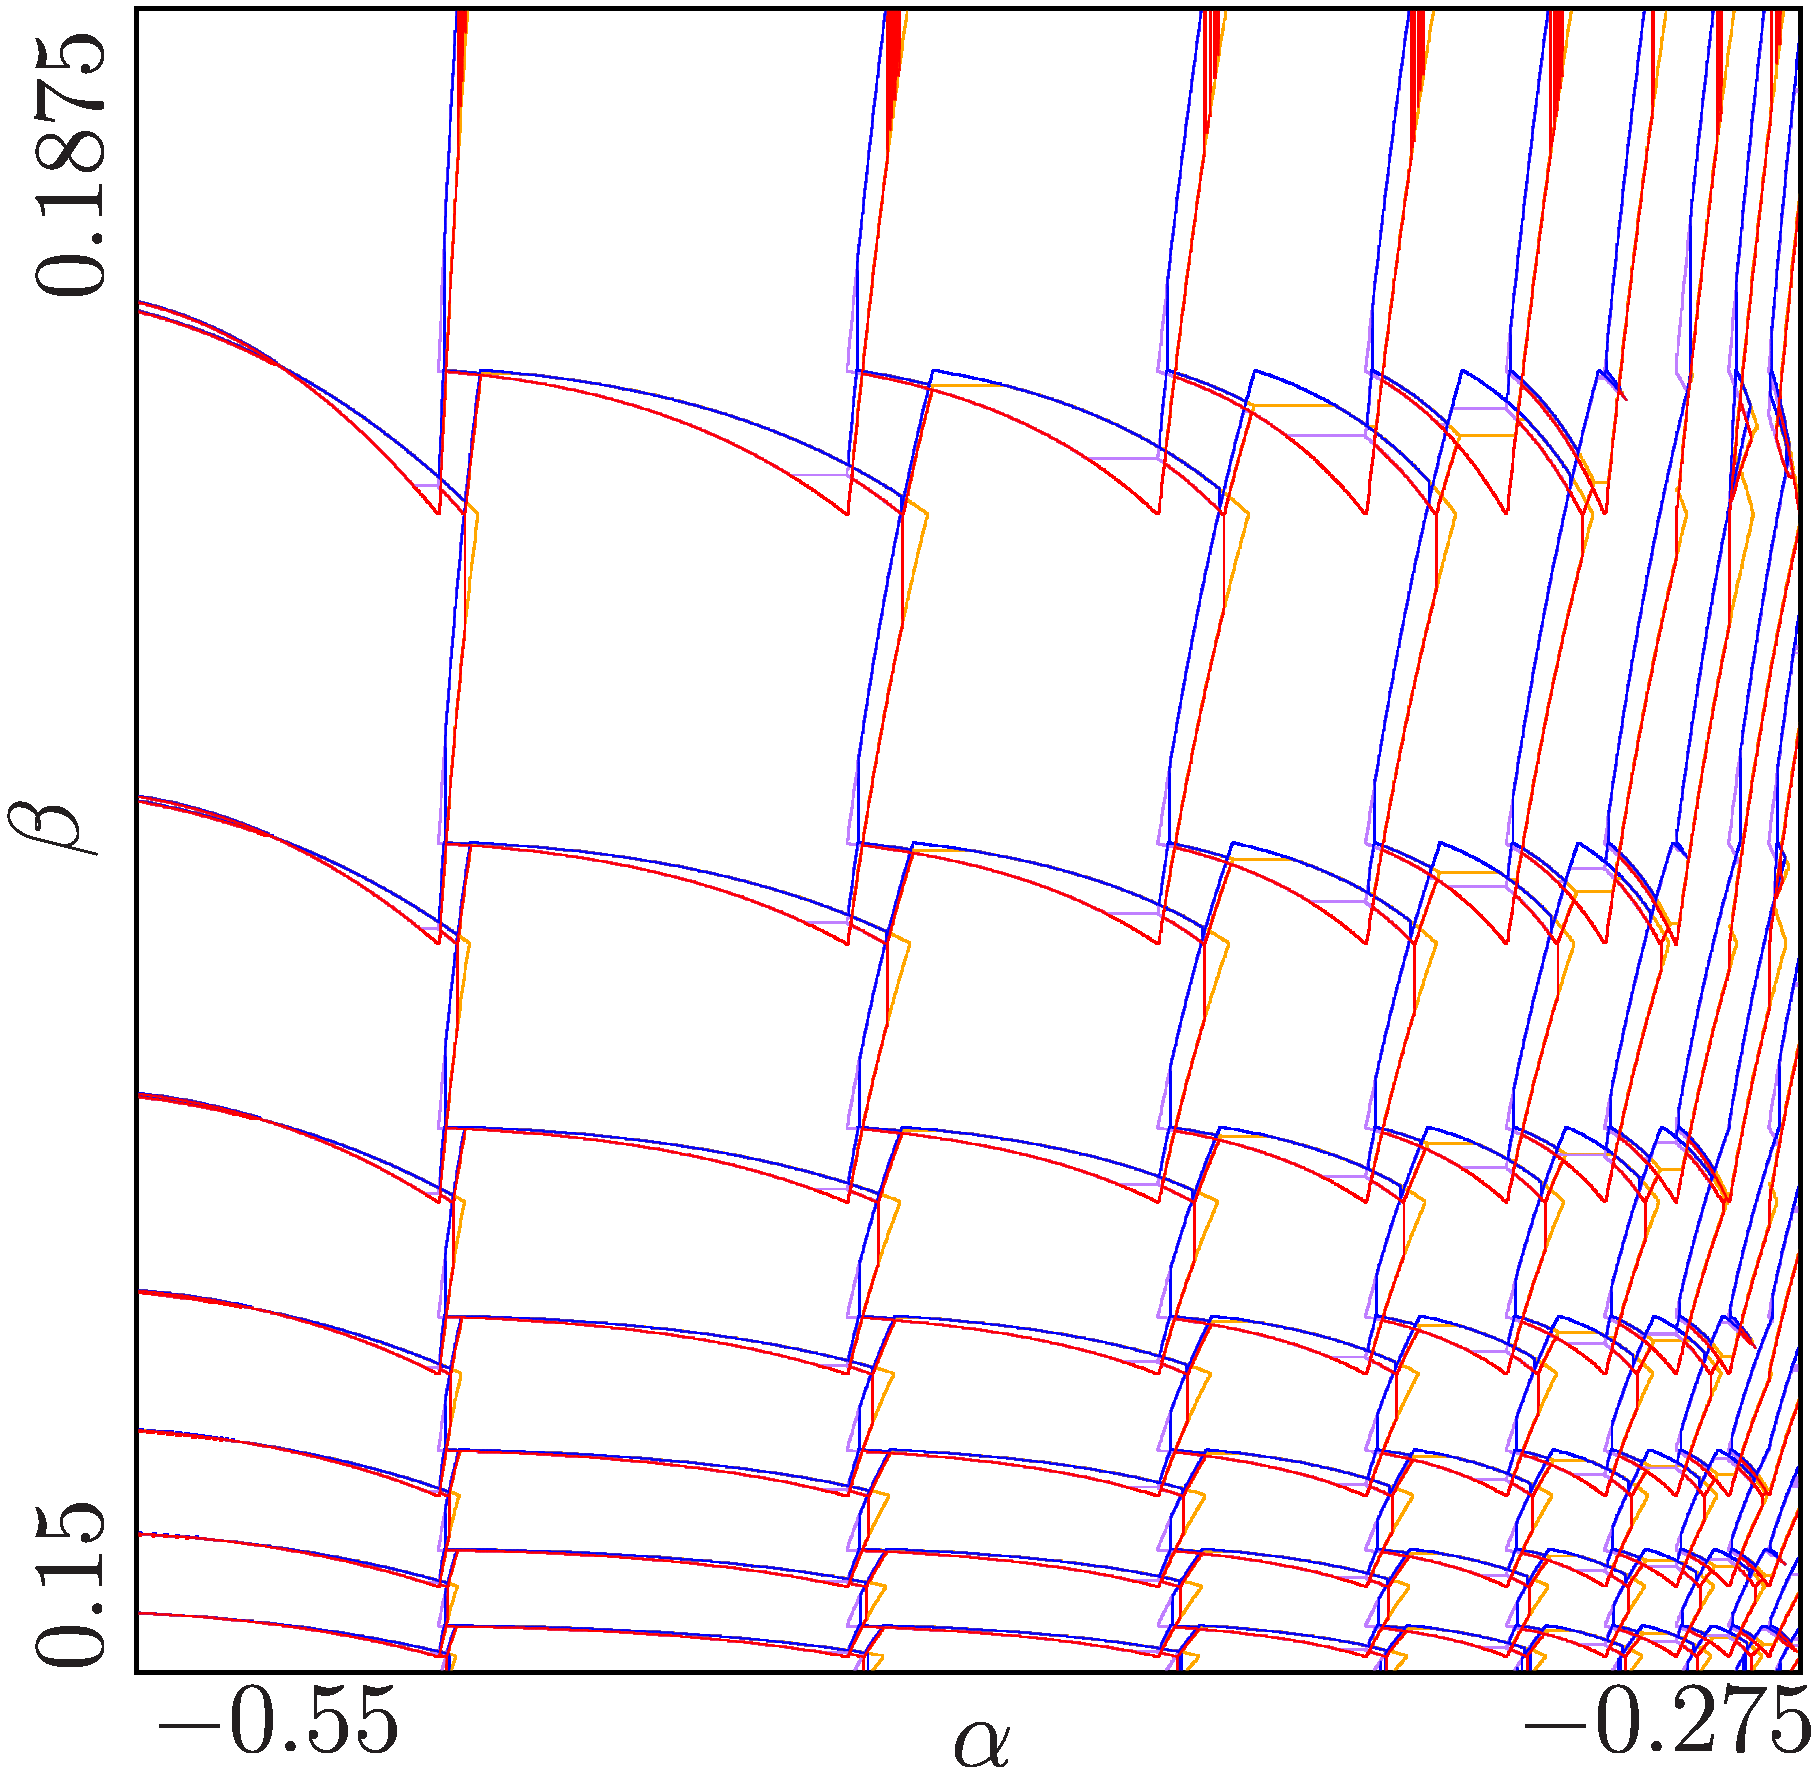
\includegraphics[width=.4 \textwidth]{../Figures/6/6.3a/result.png}
		\label{fig:arch.dyn.regions.full}
	}
	\subfloat[Zoomed-in]{
		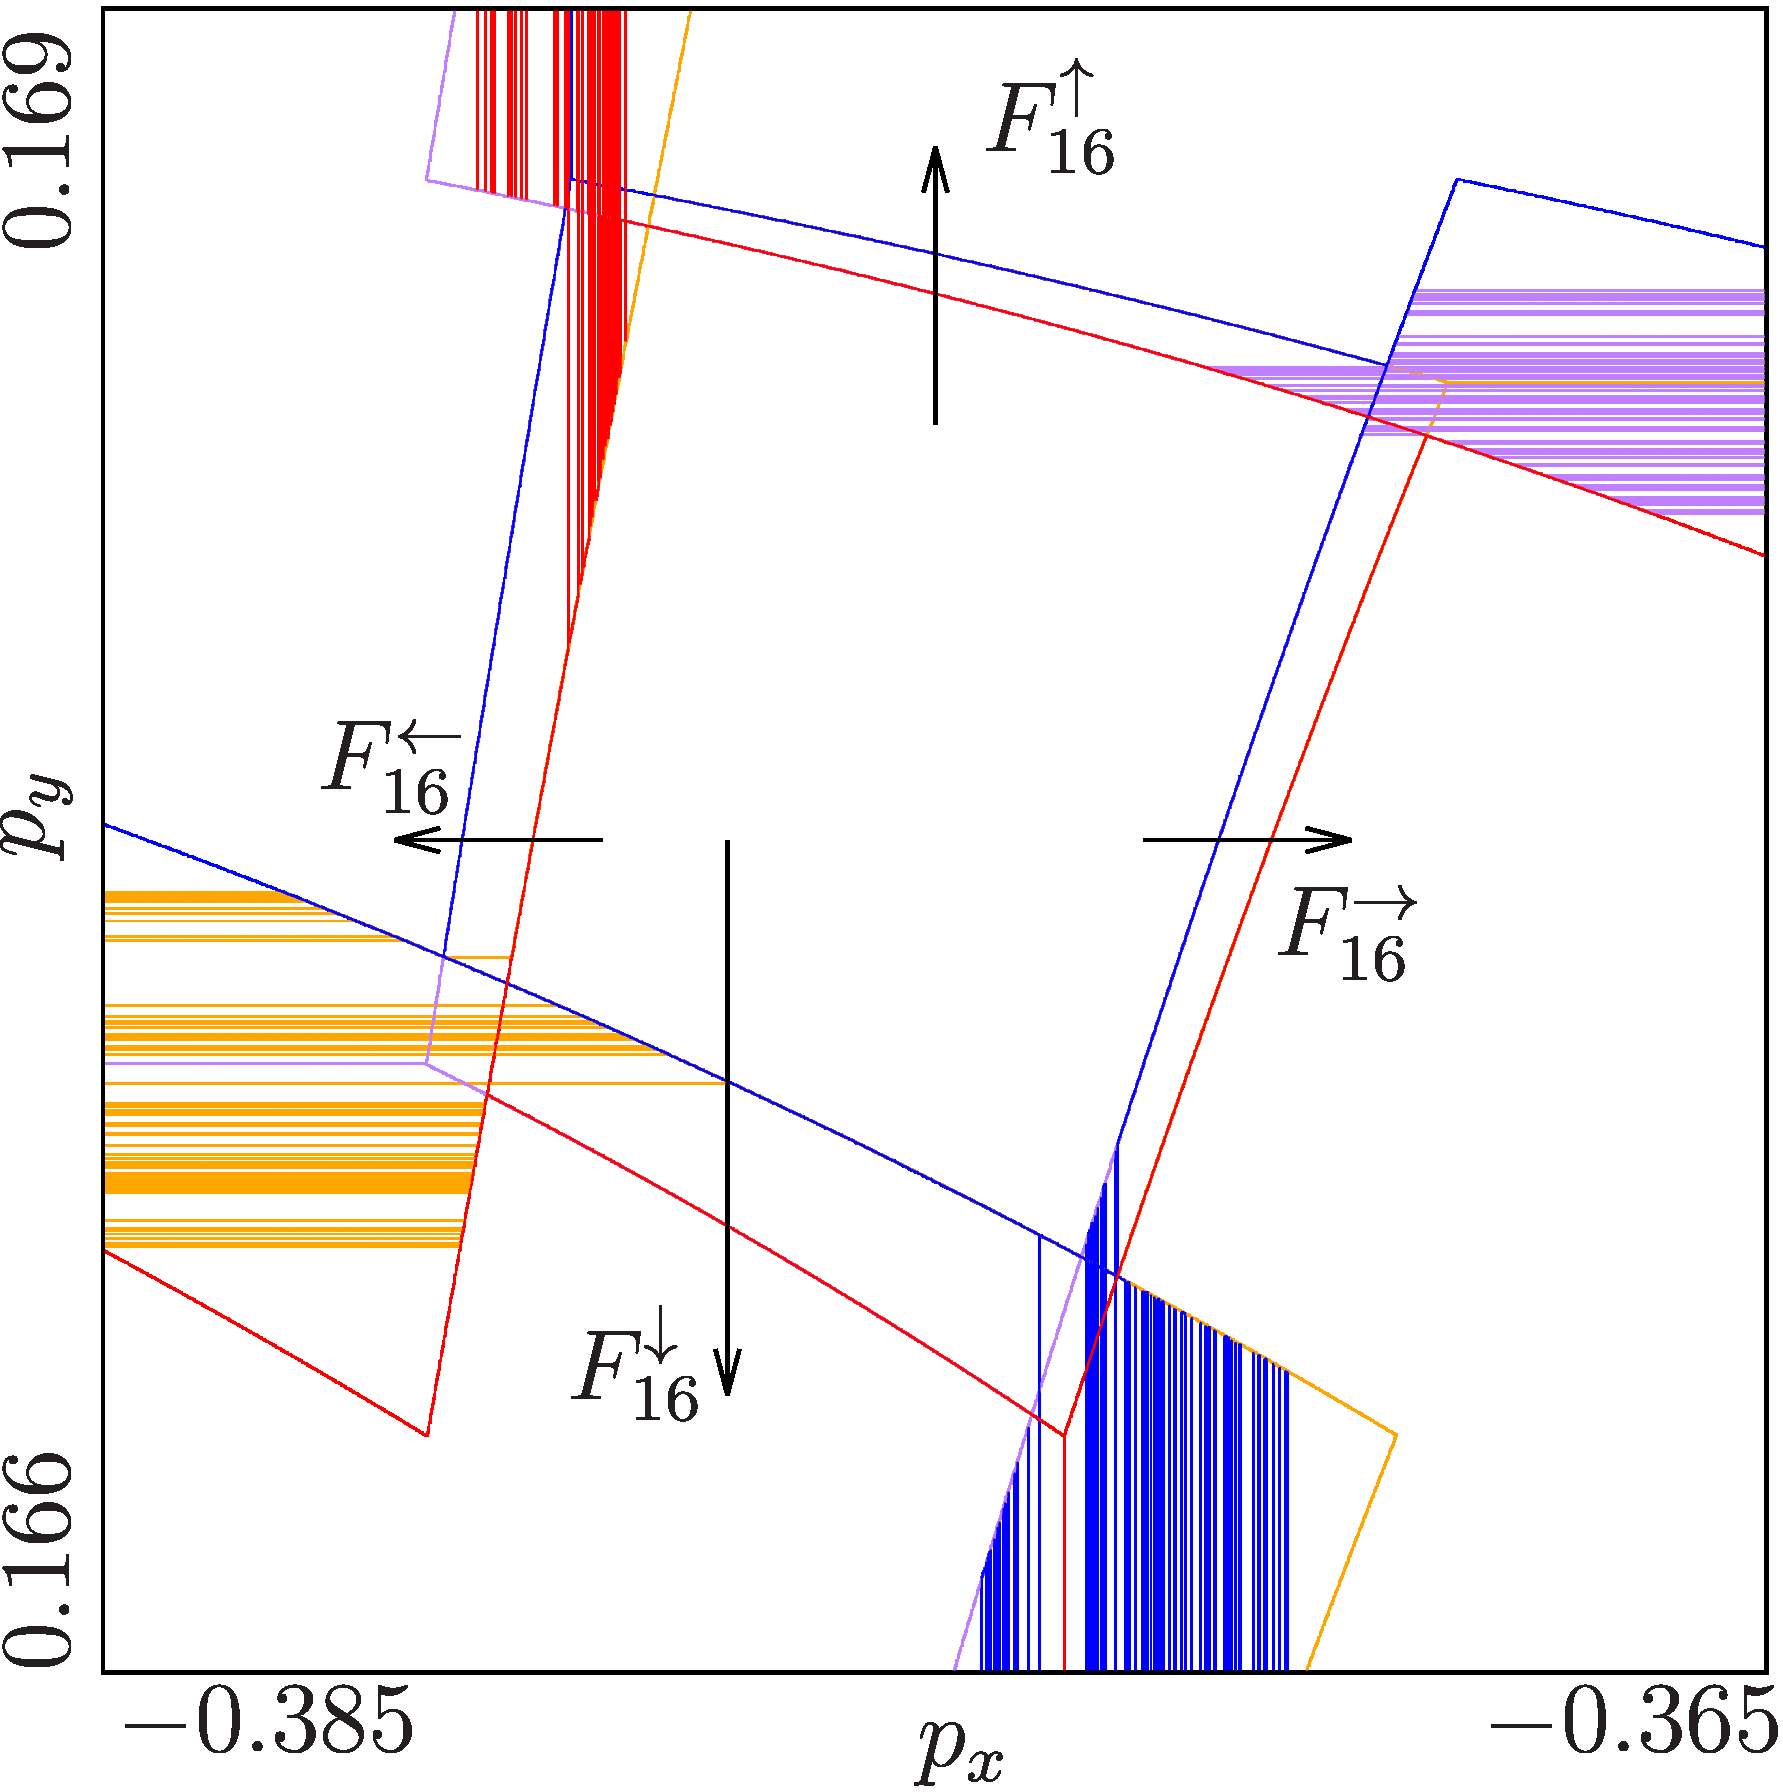
\includegraphics[width=.4 \textwidth]{../Figures/6/6.3b/result.png}
		\label{fig:arch.dyn.regions.zoomed}
	}
	\caption[2D scans of the boundaries of parameter regions with different symbolic sequences in the archetypal model]{
		2D scans of the boundaries of parameter regions with different symbolic sequences in the archetypal model.
		The parameters $a_L = 4, b_L = -\frac{1}{2},$ and $g_R\left(\frac{1}{2}\right) = \frac{1}{2} + \frac{1}{40}$ are fixed.
		The parameters $\alpha = -g_R\left(\frac{1}{4}\right)$ and $\beta = c_L$ are varied in different ranges.
		(a) shows full version with the parameters being varied in the ranges $[-0.55, -0.275]$ and $[0.15, 0.1875]$.
		(b) shows the zoomed-in version with the parameters being varied in the ranges $[-0.385, -0.365]$ and $[0.166, 0.169]$.
		It focuses on the ``type B'' parameter region marked with point $F_{16}$ in \Cref{fig:arch.dyn.period}.
		Its boundaries are marked with $F_{16}^\uparrow, F_{16}^\downarrow, F_{16}^\leftarrow,$ and $F_{16}^\rightarrow$.
	}
	\label{fig:arch.dyn.regions}
\end{figure}

\section{Bifurcations}
\label{sec:arch.bif}

This section explores the bifurcations that happen at the borders of ``type A'' and ``type B'' parameter regions, respectively.
\Cref{fig:arch.dyn.regions.full} shows the borders of the parameter regions in full.
\Cref{fig:arch.dyn.regions.zoomed} is a zoomed-in version that pictures the parameter region that contains the point $F_{16}$ of \Cref{fig:arch.dyn.period}.
It is a ``type B'' parameter region with the stable cycles $\Cycle{\A^5\B^3\C^4\D^4}$ and $\Cycle{\A^4\B^4\C^5\D^3}$.
Every one of its boundaries has a ``type A'' parameter region on the other side.
Therefore, this section only describes the four boundaries of this ``type B'' parameter region in depth to cover all the boundaries of both ``type A'' and ``type B'' parameter regions.

The boundaries of the parameter region containing $F_{16}$ are named $F_{16}^\uparrow$ for the upper boundary, $F_{16}^\downarrow$ for the lower boundary, $F_{16}^\leftarrow$ for the left boundary, and finally $F_{16}^\rightarrow$ for the right boundary.
These boundaries are also marked with arrows in \Cref{fig:arch.dyn.regions.zoomed}.
The first boundary that is covered is $F_{16}^\uparrow$.

\subsection{The Boundary $F_{16}^\uparrow$}
\label{sec:arch.bif.U}

\begin{figure}
	\centering
	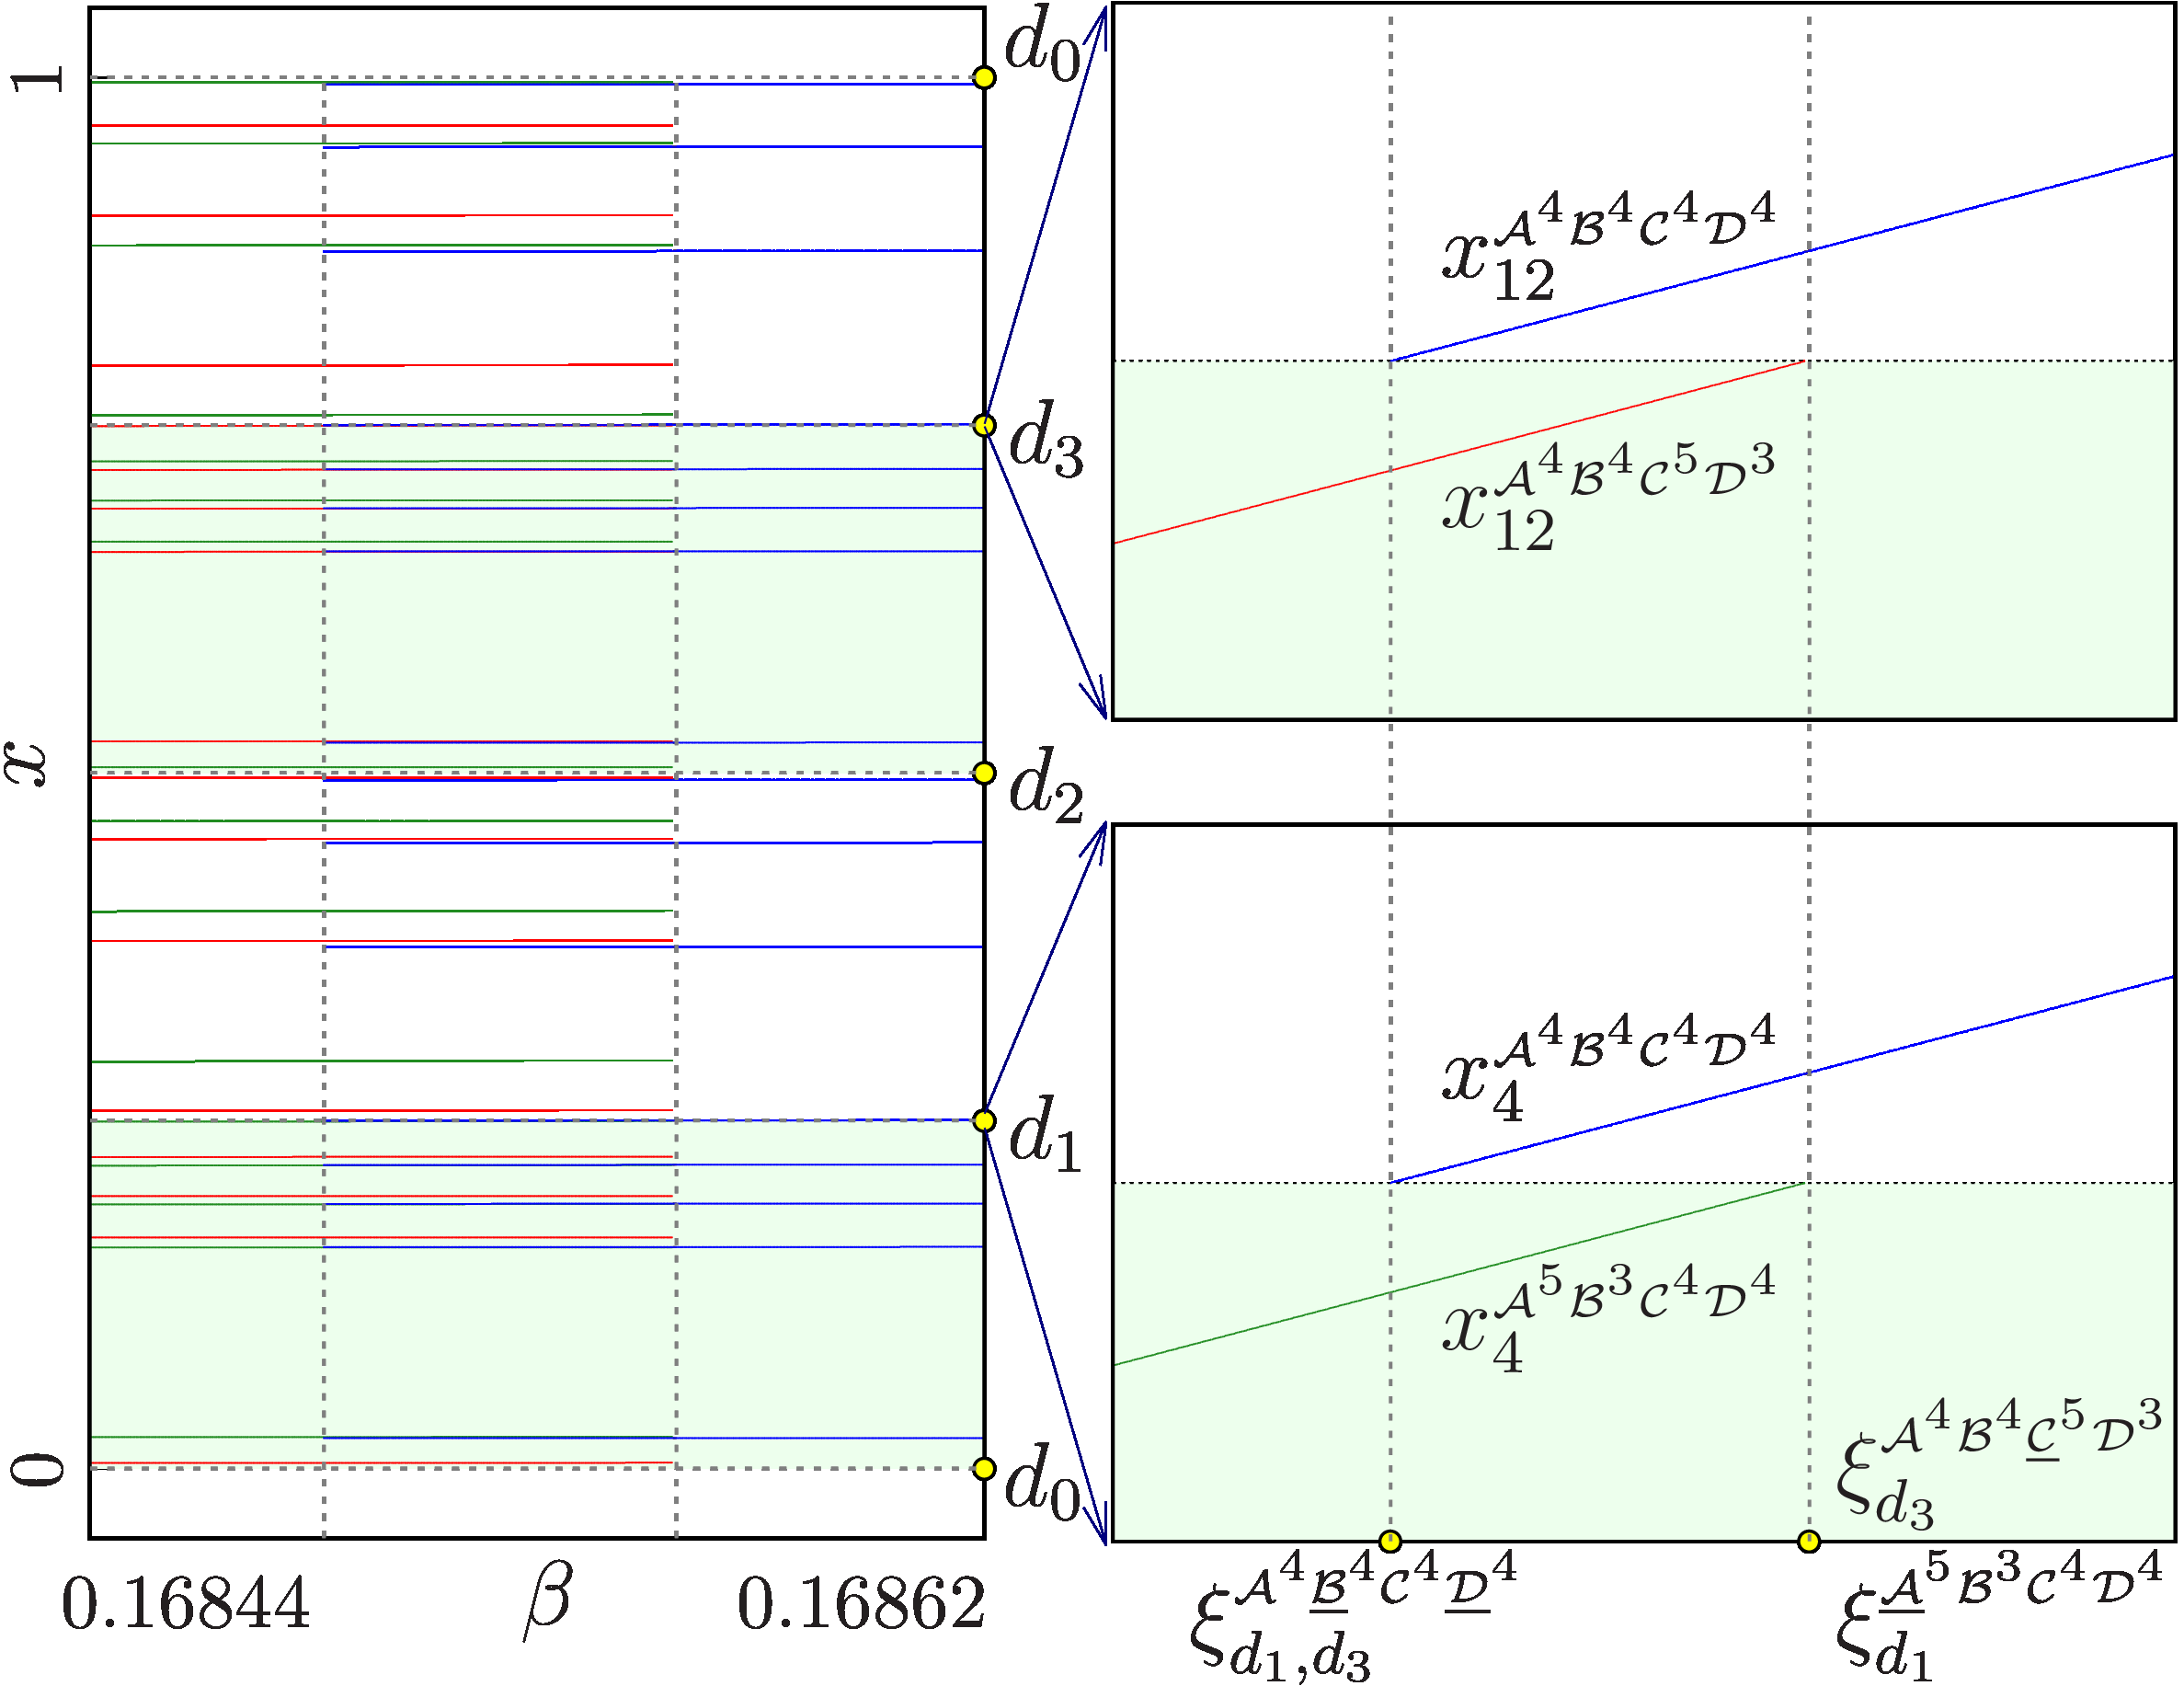
\includegraphics[width=.7 \textwidth]{../Figures/6/6.4/result.png}
	\caption[1D bifurcation diagram at the boundary $F_{16}^\uparrow$ in the archetypal model]{
		1D bifurcation diagram at the boundary $F_{16}^\uparrow$ in the archetypal model.
		The parameters $a_L = 4, b_L = -\frac{1}{2}, g_R\left(\frac{1}{2}\right) = \frac{1}{2} + \frac{1}{40},$ and $\alpha = -g_R\left(\frac{1}{4}\right) = -0.375$ are fixed.
		The parameter $\beta = c_L$ is varied in the range $[0.16844, 0.16862]$ marked with an arrow in \Cref{fig:arch.dyn.regions.zoomed}.
		On the left, the whole state space is pictured while the right side enhances the area of the state space around the borders involved in the pictured border collision bifurcations.
	}
	\label{fig:arch.bif.F.up}
\end{figure}

\Cref{fig:arch.bif.F.up} shows the bifurcation diagram of the first considered boundary, $F_{16}^\uparrow$.
To better differentiate between the two coexisting ``type B'' cycles of the parameter region marked with point $F_{16}$, they are plotted in different colors.
The cycle $\Cycle{\A^5\B^3\C^4\D^4}$ is shown in green and its twin cycle $\Cycle{\A^4\B^4\C^5\D^3}$ is shown in  red.
One can see that the cycle $\Cycle{\A^5\B^3\C^4\D^4}$ shown in green collides with the border $d_1$ when it vanishes.
To be more precise, the point $x_4^{\A^5\B^3\C^4\D^4}$ which is the 5th point of the cycle $\Cycle{\A^5\B^3\C^4\D^4}$ collides with the border $d_1$.
This is a border collision bifurcation, and it is denoted as $\BCB_{d_1}^{\underline{\A}^5\B^3\C^4\D^4}$.

The lower index of $\BCB$ indicates the border of the model function that is involved in the bifurcation.
The upper index of $\BCB$ indicates two things.
First, the object that collides with the border of the model function.
In our case this is the cycle $\Cycle{\A^5\B^3\C^4\D^4}$.
Second, the underlined symbol indicates the branch of the model function, the colliding point of the cycle belongs to.
Together with the information which border is involved in the border collision bifurcation, one can determine which point of the cycle collided with the border.
For example, we know that a point of the cycle on branch $f_\A$ collides with the border $d_1$, which is the right border of the branch $f_\A$.
Since there are $5$ points on branch $f_\A$, we can derive that the point $x_4^{\A^5\B^3\C^4\D^4}$ is involved in the border collision bifurcation.

A similar thing that happens to cycle $\Cycle{\A^5\B^3\C^4\D^4}$ shown in green in \Cref{fig:arch.bif.F.up} happens to its twin cycle $\Cycle{\A^4\B^4\C^5\D^3}$ \href{shown in} red but shifted by $\frac{1}{2}$ in the state space because of the symmetry in the model.
Here, the point $x_{12}^{A^4\B^4\C^5\D^3}$ collides with the border $d_3$ and the bifurcation is denoted as $\BCB_{d_3}^{A^4\B^4\underline{\C}^5\D^3}$.
In both cases, the cycles collide from the left side of the border.

The ``type A'' parameter region above is $\P_{\A^4\B^4\C^4\D^4}$.
The cycle $\Cycle{\A^4\B^4\C^4\D^4}$ shown in blue, which is stable in that parameter region, collides with the same borders the ``type B'' cycles collide with, $d_1$ and $d_3$.
But here, two points of the same cycle collide with two different borders at the same parameter values.
Point $x_{4}^{A^4\B^4\C^4\D^4}$ collides with the border $d_1$ while point $x_{12}^{A^4\B^4\C^4\D^4}$ collides with $d_3$.
Both collisions happen from the right side of the borders.
So one point of the cycle on the branch $f_{\B}$ collides with $d_1$ and one point on the branch $f_{\D}$ collides with $d_3$.
This is unusual for border collision bifurcations but is explained by the symmetry of both the cycle and the model function.
The bifurcation is denoted as $\BCB_{d_1, d_3}^{\A^4\underline{\B}^4\C^4\underline{\D}^4}$.

\subsection{The Boundary $F_{16}^\downarrow$}
\label{sec:arch.bif.D}

At the lower boundary $F_{16}^\downarrow$, the two cycles $\Cycle{\A^5\B^3\C^4\D^4}$ and $\Cycle{\A^4\B^4\C^5\D^3}$ also collide with the borders $d_1$ and $d_3$, this time from the right side of the borders.
But while the cycle $\Cycle{\A^5\B^5\C^4\D^4}$ shown in green collides with the border $d_1$ at the upper boundary, here it collides with the border $d_3$.
To be more precise, the point $x_{12}^{\A^5\B^3\C^4\D^4}$ collides with the border $d_3$.
Meaning one point on the branch $f_{\D}$ collides with the border $d_3$.
This border collision bifurcation is written as $\BCB_{d_3}^{\A^5\B^3\C^4\underline{\D}^4}$.
Similarly, the point $x_{4}^{\A^4\B^4\C^5\D^3}$ of the cycle $\Cycle{\A^4\B^4\C^5\D^3}$ shown in red now collides with the border $d_1$ from the right side of the border.
Meaning that one point of branch $f_{\B}$ collides with the border $d_1$.
This border collision bifurcation is written as $\BCB_{d_1}^{\A^4\underline{\B}^4\C^5\D^3}$.

The ``type A'' parameter region below the ``type B'' parameter region is $\P_{\A^5\B^3\C^5\D^3}$.
The cycle $\P_{\A^5\B^3\C^5\D^3}$ shown in blue collides with the same borders as the ``type B'' cycles, just like before at the upper boundary $F_{16}^\uparrow$.
Again, two points of this cycle collide with two different borders, $d_1$ and $d_2$, at the same parameter values.
But here they collide from the left side.
The point colliding with $d_1$ is $x_{4}^{A^5\B^3\C^5\D^3}$ and the point colliding with $d_3$ is $x_{12}^{A^5\B^3\C^5\D^3}$.
So one point on the branch $f_{\A}$ collides with the border $d_1$ and one point on the branch $f_{\C}$ collides with the border $d_3$.
This bifurcation is written as $\BCB_{d_1, d_3}^{\underline{\A}^5\B^3\underline{\C}^5\D^3}$.

\begin{figure}[H]
	\centering
	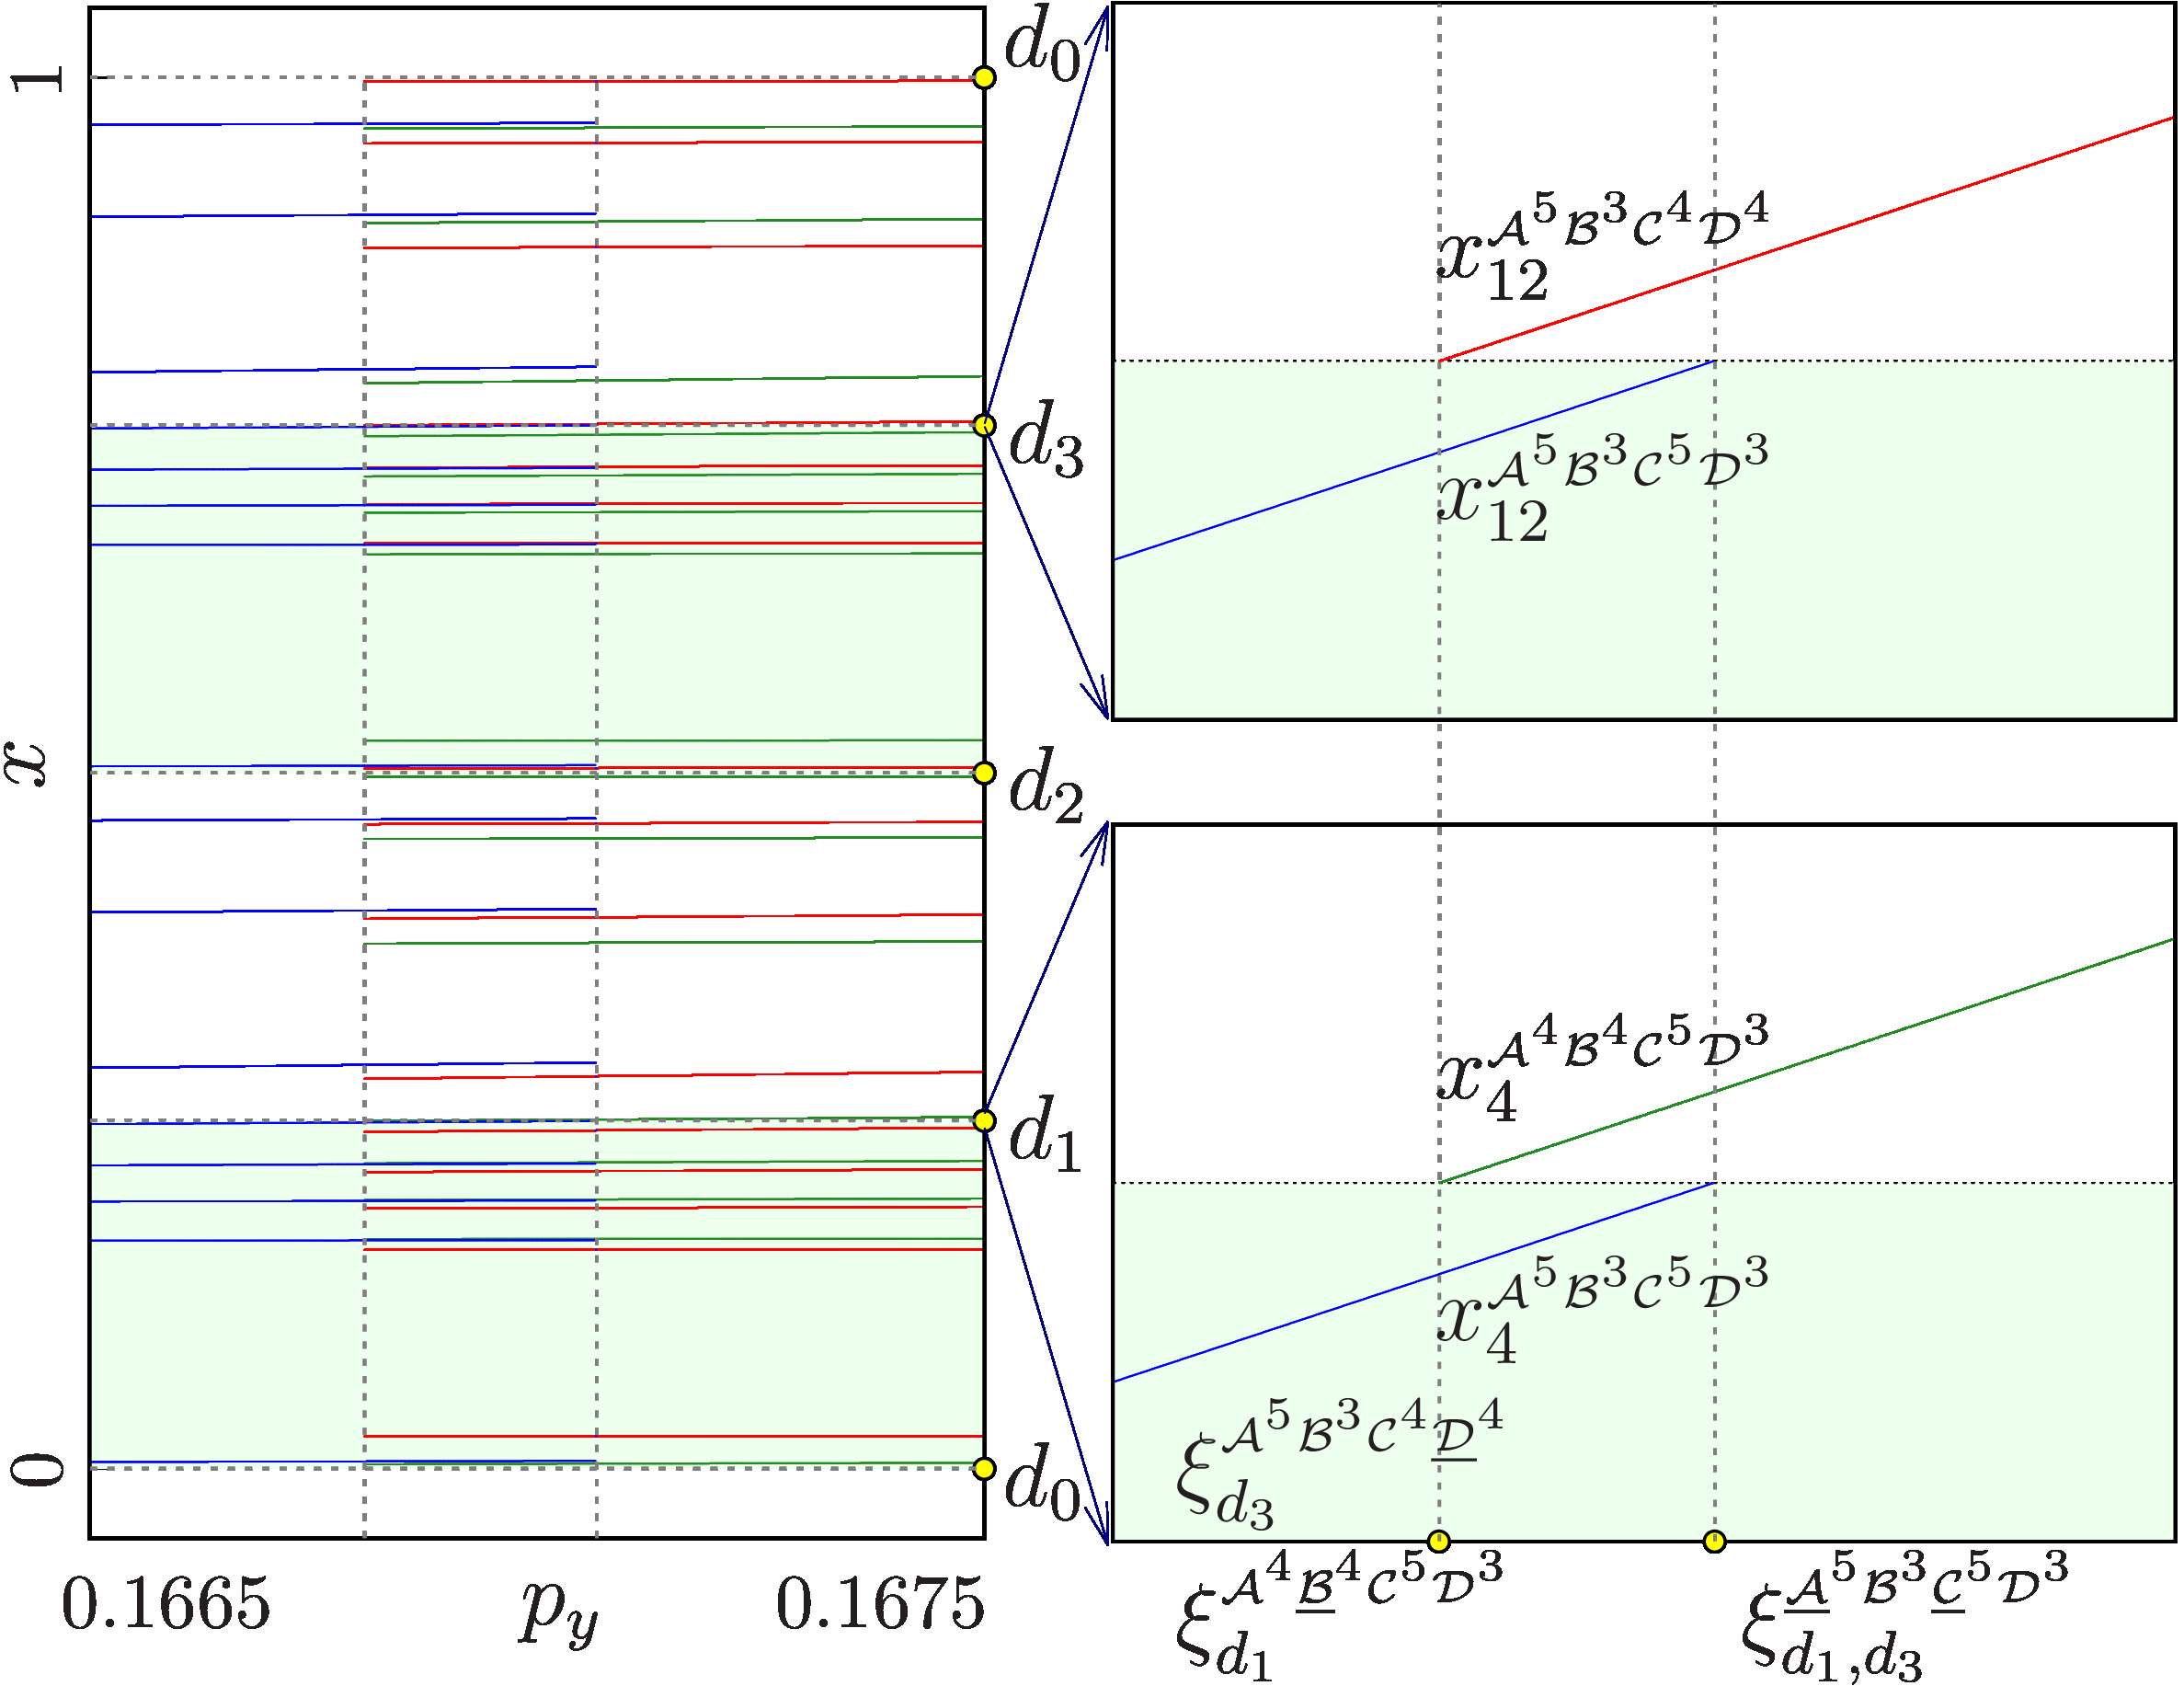
\includegraphics[width=.7 \textwidth]{../Figures/6/6.5/result.png}
	\caption[1D bifurcation diagram at the boundary $F_{16}^\downarrow$ in the archetypal model]{
		1D bifurcation diagram at the boundary $F_{16}^\downarrow$ in the archetypal model.
		The parameters $a_L = 4, b_L = -\frac{1}{2}, g_R\left(\frac{1}{2}\right) = \frac{1}{2} + \frac{1}{40},$ and $\alpha = -g_R\left(\frac{1}{4}\right) = -0.3775$ are fixed.
		The parameter $\beta = c_L$ is varied in the range $[0.1665, 0.1675]$ marked with the arrow $F_{16}^\downarrow$ in \Cref{fig:arch.dyn.regions.zoomed}.
		On the left, the whole state space is pictured while the right side enhances the area of the state space around the borders involved in the pictured border collision bifurcations.
	}
	\label{fig:arch.bif.F.down}
\end{figure}

\subsection{The Boundary $F_{16}^\leftarrow$}
\label{sec:arch.bif.L}

\begin{figure}
	\centering
	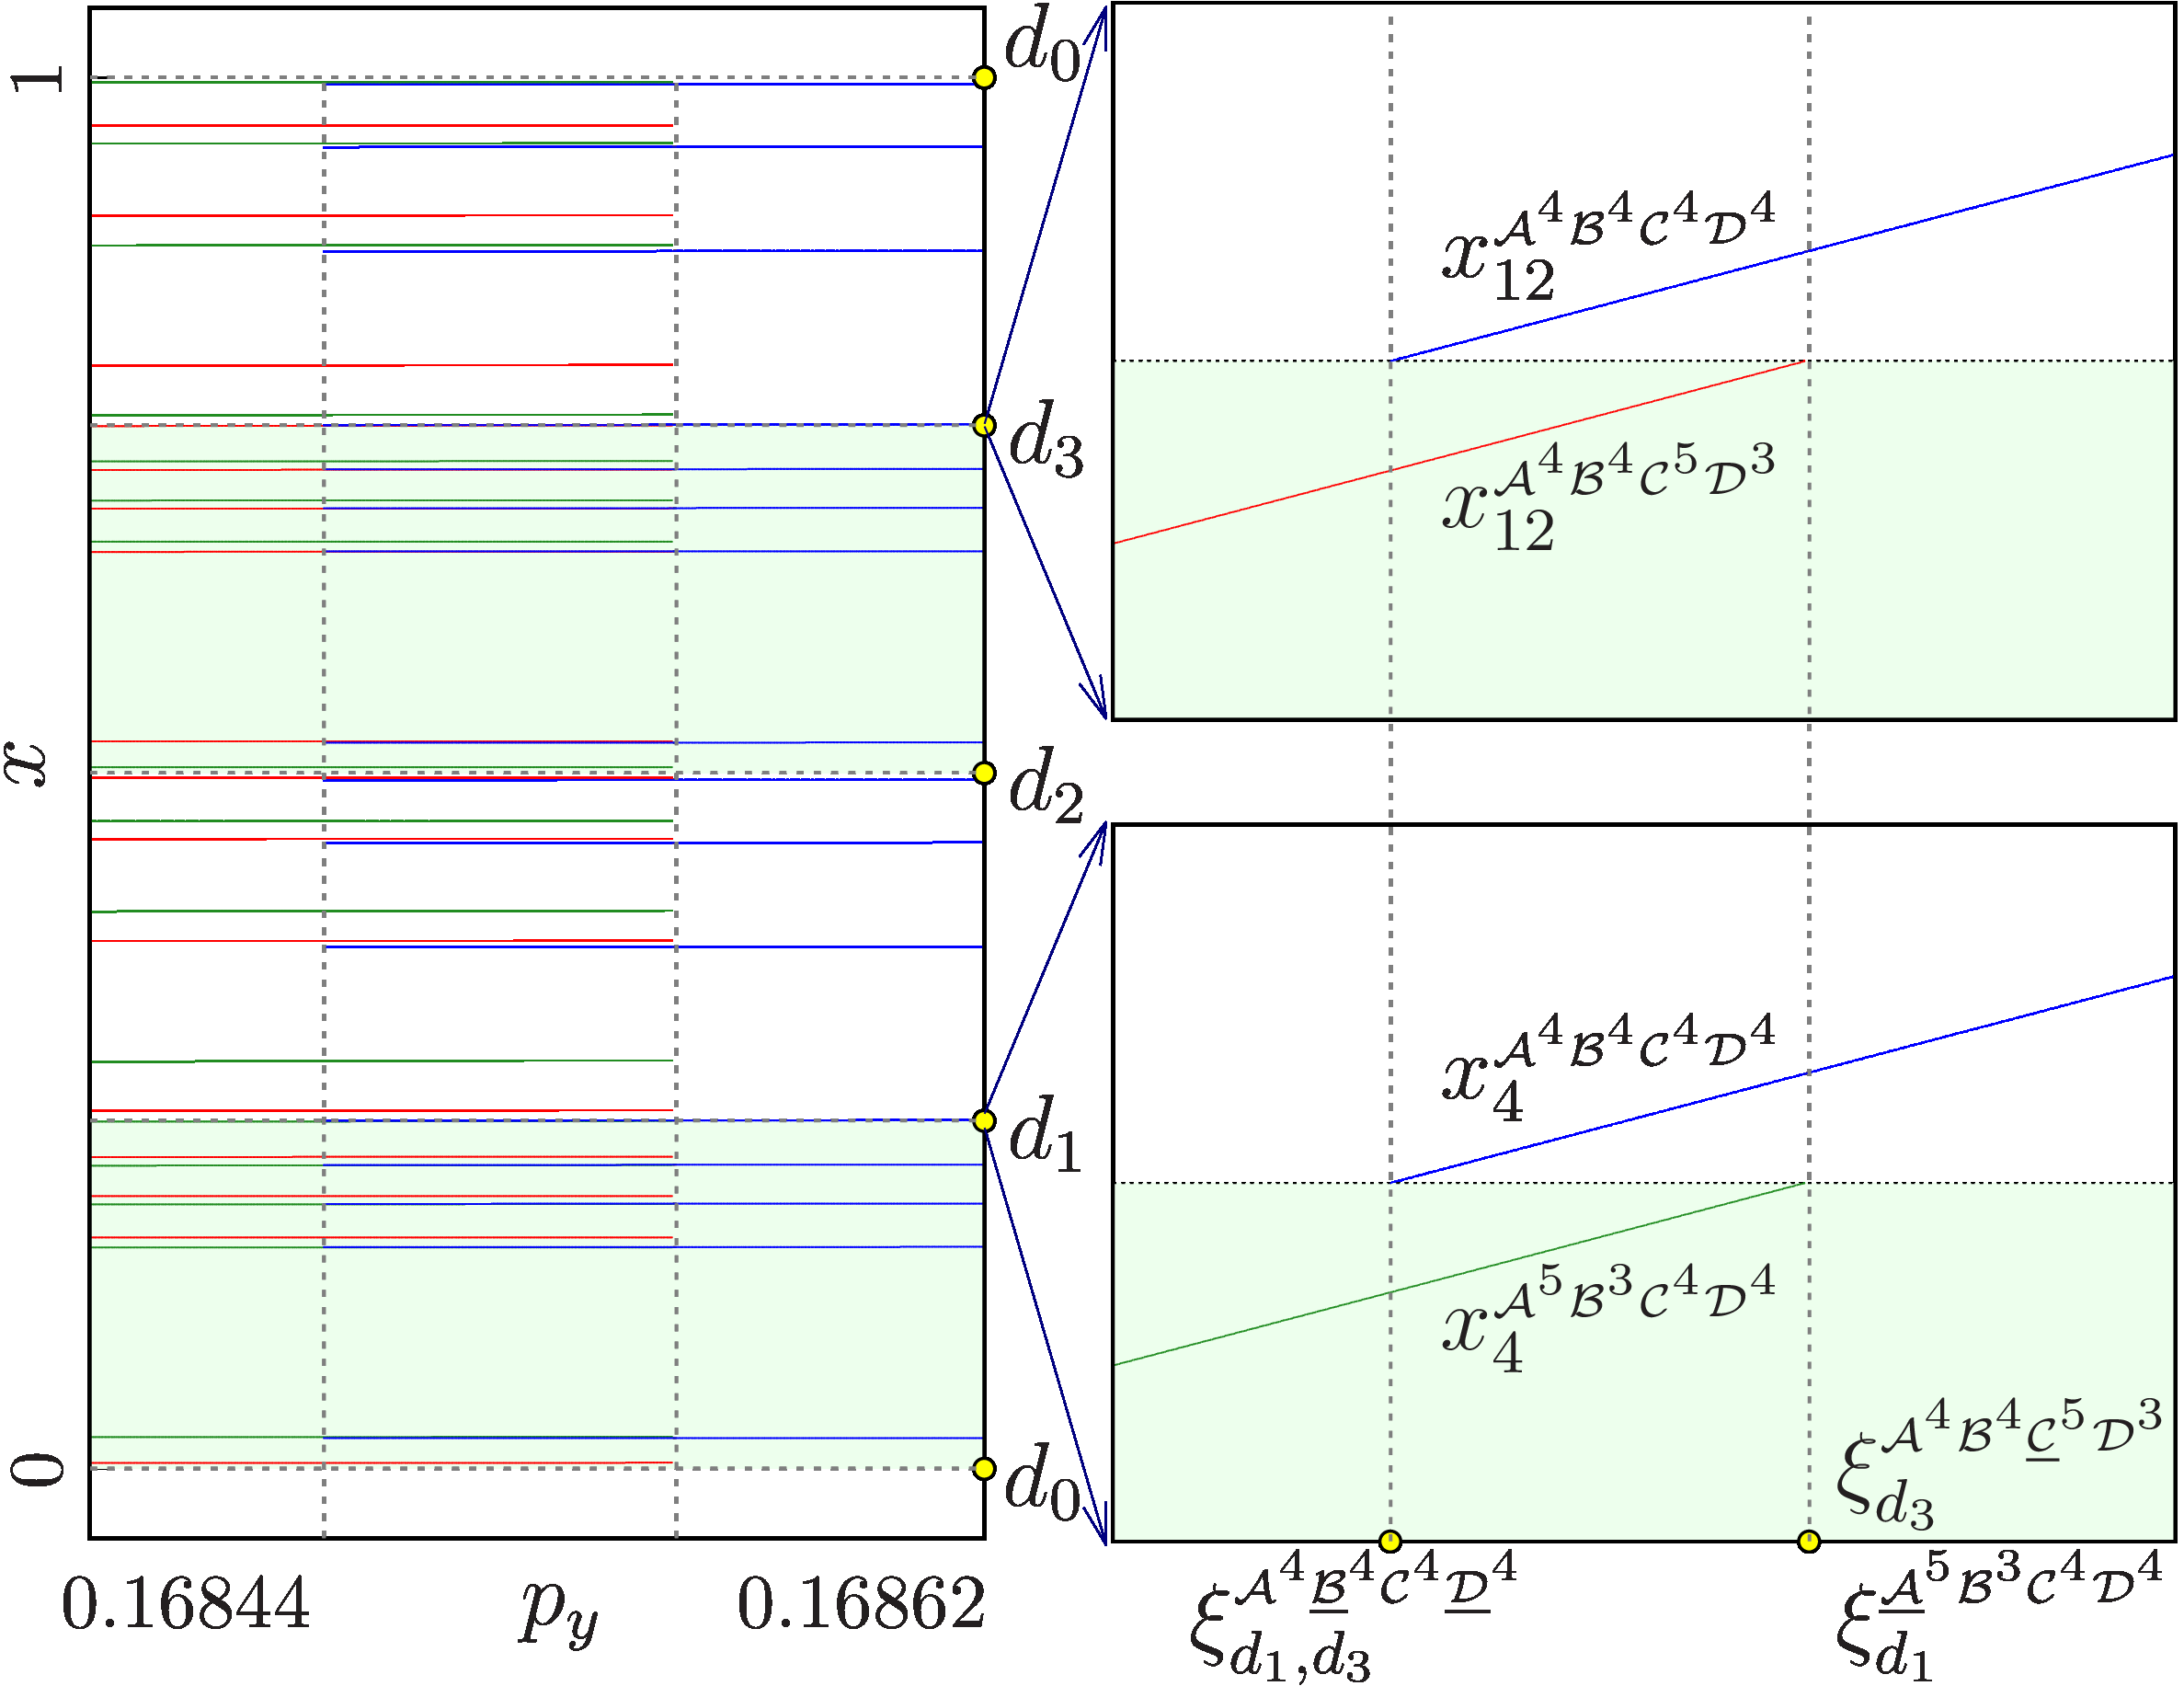
\includegraphics[width=.7 \textwidth]{../Figures/6/6.6/result.png}
	\caption[1D bifurcation diagram at the boundary $F_{16}^\leftarrow$ in the archetypal model]{
		1D bifurcation diagram at the boundary $F_{16}^\leftarrow$ in the archetypal model.
		The parameters $a_L = 4, b_L = -\frac{1}{2}, g_R\left(\frac{1}{2}\right) = \frac{1}{2} + \frac{1}{40},$ and $\beta = c_L = 0.1675$ are fixed.
		The parameter $\alpha = -g_R\left(\frac{1}{4}\right)$ is varied in the range $[-0.3815, -0.379]$ marked with the arrow $F_{16}^\leftarrow$ in \Cref{fig:arch.dyn.regions.zoomed}.
		On the left, the whole state space is pictured while the right side enhances the area of the state space around the borders involved in the pictured border collision bifurcations.
	}
	\label{fig:arch.bif.F.left}
\end{figure}

The next examined boundaries are the horizontal boundaries of the same parameter region.
At the left boundary $F_{16}^\leftarrow$, the two cycles $\Cycle{\A^5\B^3\C^4\D^4}$ shown in green in \Cref{fig:arch.bif.F.left} and $\Cycle{\A^4\B^4\C^5\D^3}$ shown in red collide with the borders $d_1$ and $d_2$ from the right.
These are different borders than the borders involved in the border collision bifurcations at the vertical boundaries $F_{16}^\uparrow$ and $F_{16}^\downarrow$.
The point $x_{7}^{\A^4\B^4\B^5\D^3}$, which is on branch $f_{\B}$, collides with $d_2$ while the point $x_{15}^{\A^5\B^3\C^4\D^4}$, which is on branch $f_{\D}$, collides with the border $d_0$.
These bifurcations are written $\BCB_{d_0}^{\A^5\underline{\B}^3\C^4\D^4}$ and $\BCB_{d_2}^{\A^4\B^4\C^5\underline{\D}^3}$ respectively.

The parameter region left to the ``type B'' parameter region is $\P_{\A^4\B^3\C^4\D^3}$.
As before with the vertical boundaries $F_{16}^\uparrow$ and $F_{16}^\downarrow$, the cycle of the neighboring ``type A'' parameter region collides with the same borders as the ``type B'' cycles but from the opposite direction.
The point $x_{0}^{\A^4\B^3\C^4\D^3}$, which is on branch $f_{\A}$, collides with the border $d_0$ while the point $x_{7}^{\A^4\B^3\C^4\D^3}$, which is on branch $f_{\C}$, collides with the border $d_2$.
This bifurcation is denoted as $\BCB_{d_0, d_2}^{\A^4\B^3\C^4\D^3}$.

\subsection{The Boundary $F_{16}^\rightarrow$}
\label{sec:arch.bif.R}

\begin{figure}
	\centering
	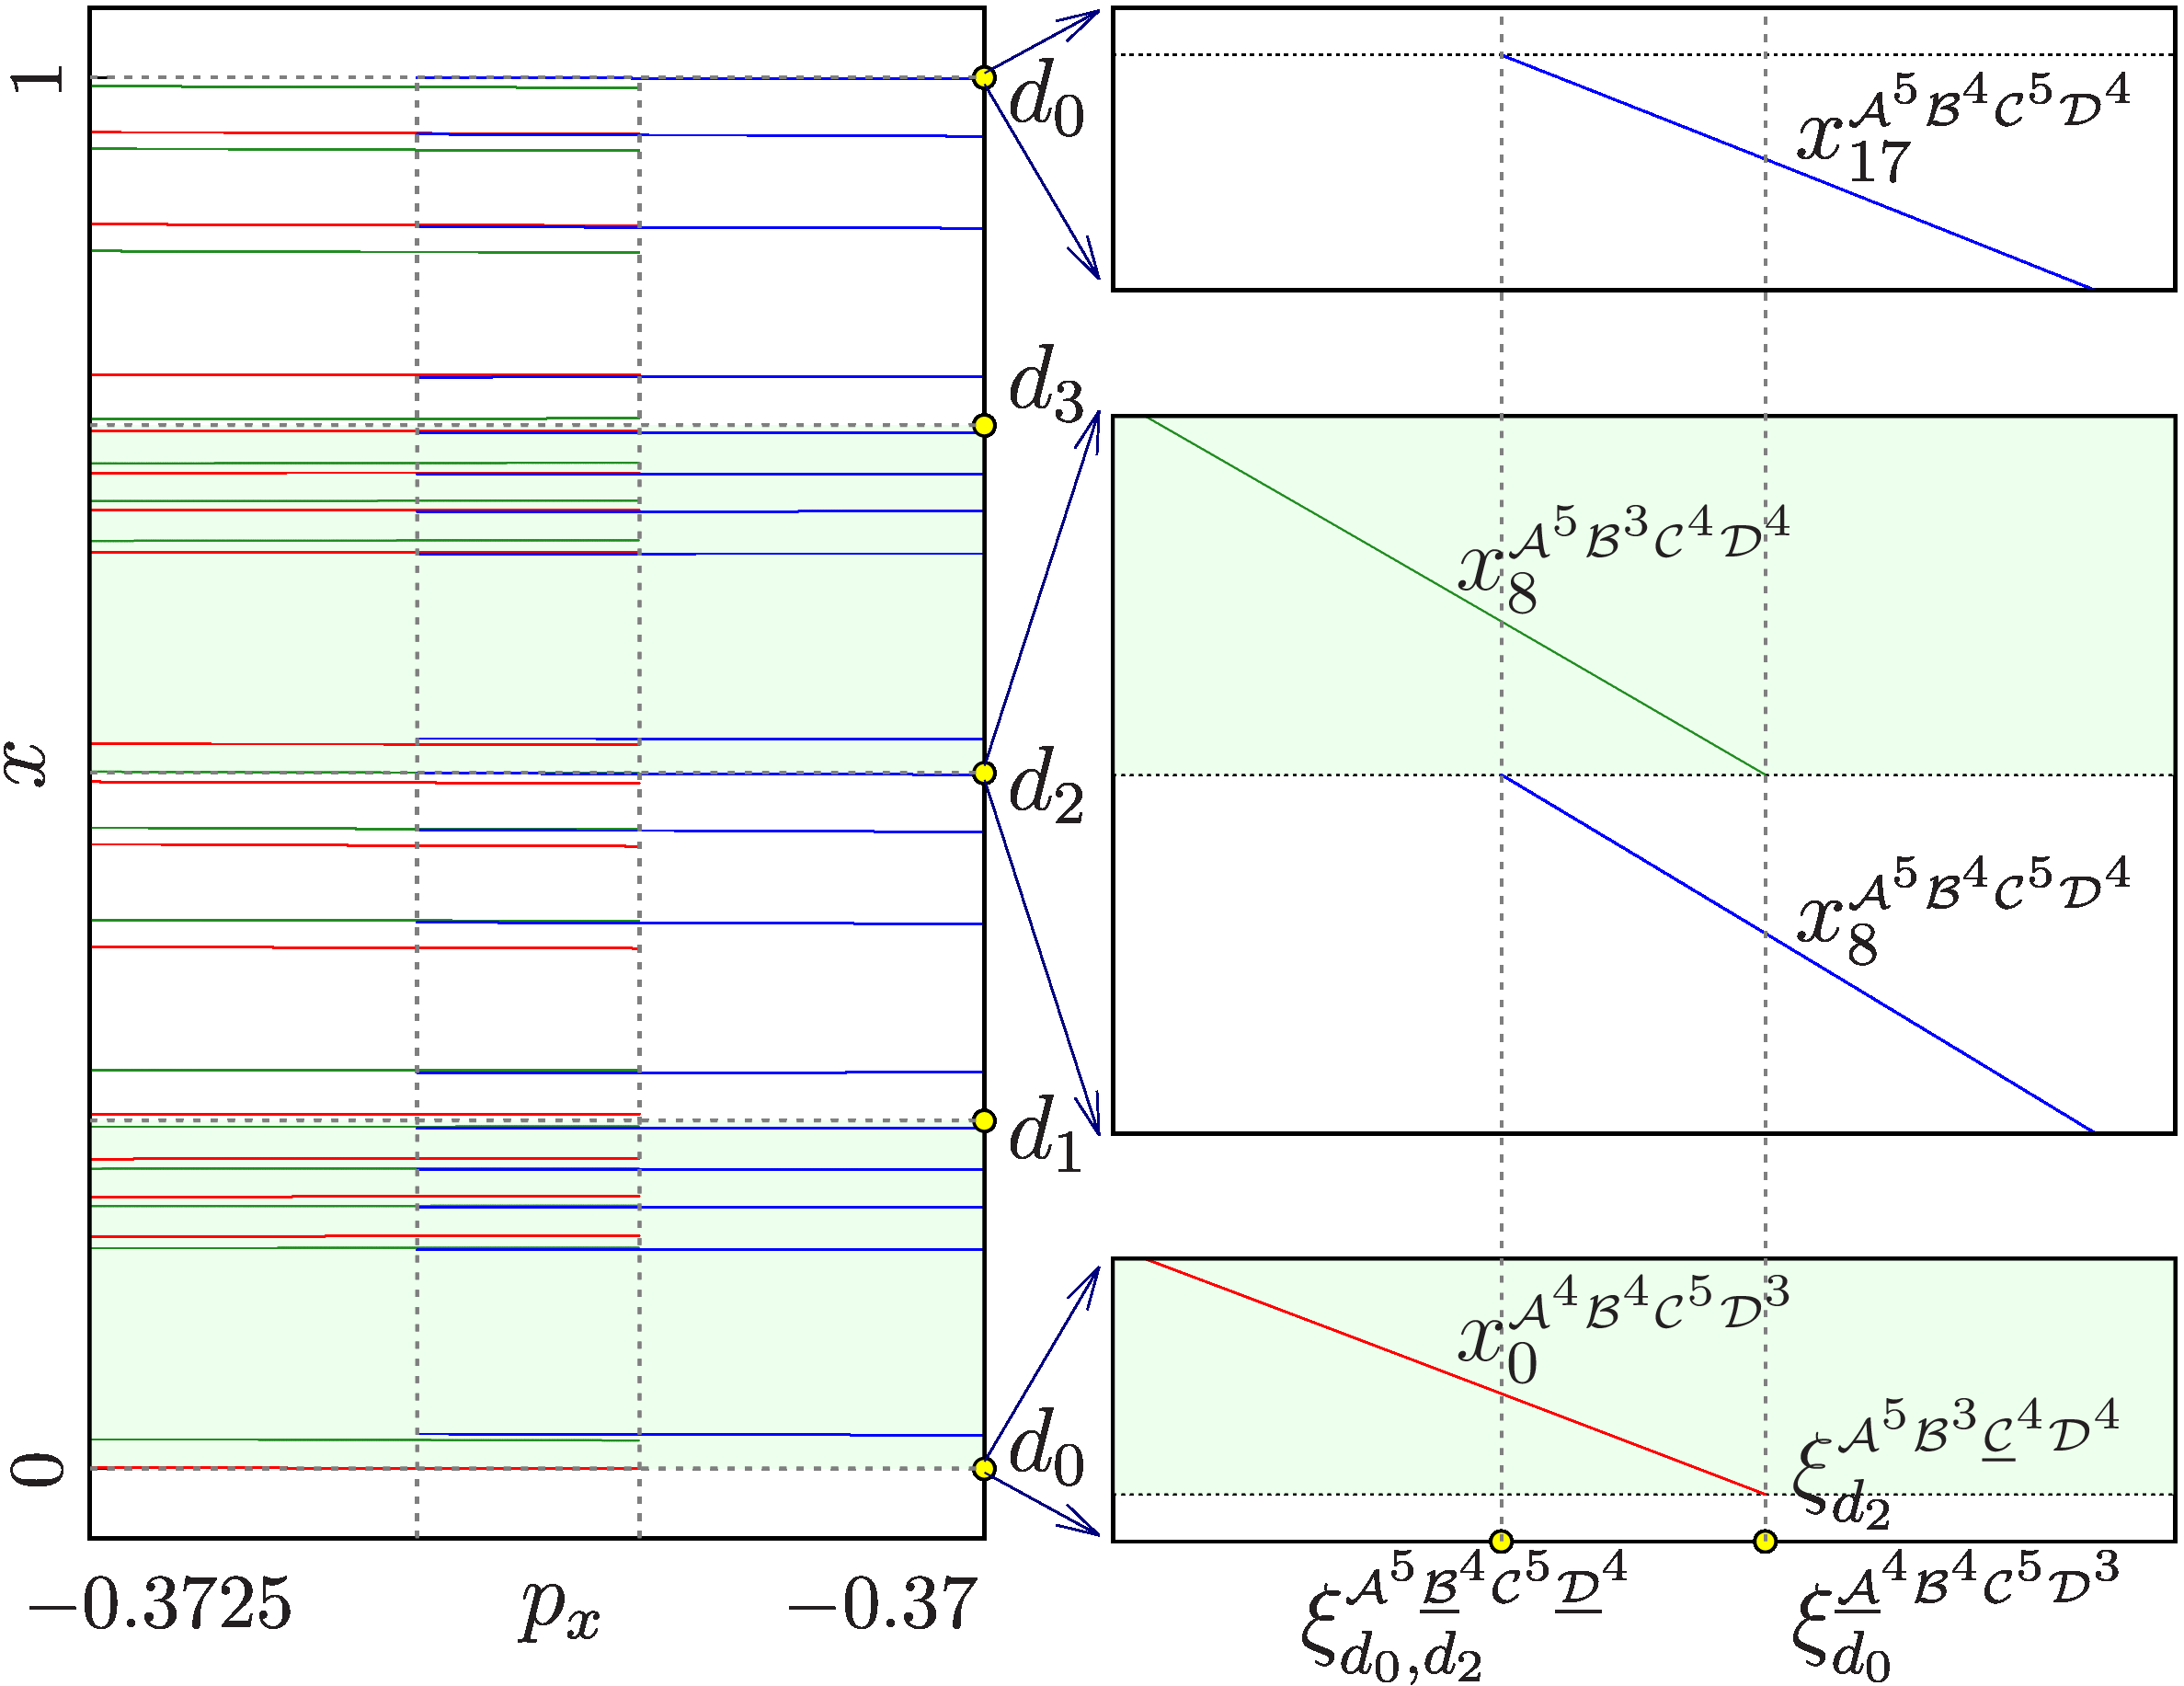
\includegraphics[width=.7 \textwidth]{../Figures/6/6.7/result.png}
	\caption[1D bifurcation diagram at the boundary $F_{16}^\rightarrow$ in the archetypal model]{
		1D bifurcation diagram at the boundary $F_{16}^\rightarrow$ in the archetypal model.
		The parameters $a_L = 4, b_L = -\frac{1}{2}, g_R\left(\frac{1}{2}\right) = \frac{1}{2} + \frac{1}{40},$ and $\beta = c_L = 0.1675$ are fixed.
		The parameter $\alpha = -g_R\left(\frac{1}{4}\right)$ is varied in the range $[-0.3725, -0.37]$ marked with the arrow $F_{16}^\rightarrow$ in \Cref{fig:arch.dyn.regions.zoomed}.
		On the left, the whole state space is pictured while the right side enhances the area of the state space around the borders involved in the pictured border collision bifurcations.
	}
	\label{fig:arch.bif.F.right}
\end{figure}

At the right boundary $F_{16}^\rightarrow$, the two cycles $\Cycle{\A^5\B^3\C^4\D^4}$ shown in green in \Cref{fig:arch.bif.F.right} and $\Cycle{\A^4\B^4\C^5\D^3}$ shown in red collide with the borders $d_0$ and $d_2$ from left of the borders.
The first point of cycle $\Cycle{A^4B^4\C^5\D^3}$ shown in green $x_{0}^{\A^4\B^4\C^5\D^3}$ collides with the border $d_0$, while the point $x_{8}^{\A^5\B^3\C^4\D^4}$ of its twin cycle $\Cycle{\A^5\B^3\C^4\D^4}$ shown in red collides with the border $d_2$.
This means that one point of the cycle $\Cycle{\A^4\B^4\C^5\D^3}$ shown in green on the branch $f_{\A}$ collides with the border $d_0$ and one point of the cycle $\Cycle{\A^5\B^3\C^4\D^4}$ shown in red on the branch $f_{\C}$ collides with the border $d_2$.
The bifurcations are written as $\BCB_{d_2}^{\A^5\B^3\underline{\C}^4\D^4}$ and $\BCB_{d_0}^{\underline{\A}^4\B^4\C^5\D^3}$, respectively.

The ``type A'' parameter region right of this parameter region is $\P_{\A^5\B^4\C^5\D^4}$.
Here again collides the ``type A'' cycle with the same borders as the ``type B'' cycles but from the opposite direction.
In this case, two of the points of the cycle $\Cycle{\A^5\B^4\C^5\D^4}$ shown in blue collide with the borders $d_0$ and $d_1$ at the same parameter value from left of the borders.
To be more precise, the point $x_{17}^{\A^5\B^4\C^5\D^4}$, which is on the branch $f_{\D}$, collides with the border $d_0$ while the point $x_{8}^{\A^5\B^4\C^5\D^4}$, which is on the branch $f_{\B}$, collides with the border $d_2$.
This bifurcation is written as $\BCB_{d_0, d_2}^{\A^5\underline{\B}^4\C^5\underline{\D}^4}$.

\subsection{Summary of Rules for Bifurcations}
\label{sec:arch.bif.sum}

In the previous sections, the bifurcations occurring at the boundaries of the considered ``type B'' boundary are distributed on many pages.
So it is hard to see regularities in the border collision bifurcations.
Also, the bifurcations of the neighboring ``type A'' parameter regions are in another order --- they are paired with the border collision bifurcation of the ``type B'' parameter region in the opposite direction.
This makes it even harder to see the regularities.
Thus, this section generalizes and summarizes the rules for the bifurcations at the boundaries of either type of parameter region.

\clearpage

\subsubsection{``Type A'' Parameter Regions}

Let the stable cycle in a ``type A'' parameter region be $\Cycle{\A^a\B^b\C^a\D^b}$.
Then the border collision bifurcations occurring at the boundaries of this parameter region are given by the following rules.

\begin{enumerate}
	\item At the upper boundary there is the bifurcation $\BCB_{d_1, d_3}^{\underline{\A}^a\B^b\underline{\C}^a\D^b}$.
	\item At the lower boundary there is the bifurcation $\BCB_{d_1, d_3}^{\A^a\underline{\B}^b\C^a\underline{\D}^b}$.
	\item At the left boundary there is the bifurcation $\BCB_{d_0, d_2}^{\A^a\underline{\B}^b\C^a\underline{\D}^b}$.
	\item At the right boundary there is the bifurcation $\BCB_{d_0, d_2}^{\underline{\A}^a\B^b\underline{\C}^a\D^b}$.
\end{enumerate}

\subsubsection{``Type B'' Parameter Regions}

Let the stable cycles in the ``type B'' parameter region be $\Cycle{\A^a\B^b\C^c\D^d}$ and $\Cycle{\A^c\B^d\C^a\D^b}$, where $c = a - 1$ and $d = b + 1$.
Then the border collision bifurcations at the boundaries of this parameter region are given by the following rules.

\begin{enumerate}
	\item At the upper boundary there are the bifurcations $\BCB_{d_1}^{\underline{\A}^a\B^b\C^c\D^d}$ and $\BCB_{d_3}^{\A^c\B^d\underline{\C}^a\D^b}$.
	\item At the lower boundary there are the bifurcations $\BCB_{d_3}^{\A^a\B^b\C^c\underline{\D}^d}$ and $\BCB_{d_1}^{\A^c\underline{\B}^d\C^a\D^b}$.
	\item At the left boundary there are the bifurcations $\BCB_{d_0}^{\A^a\B^b\C^c\underline{\D}^d}$ and $\BCB_{d_2}^{\A^c\underline{\B}^d\C^a\D^b}$.
	\item At the right boundary there are the bifurcations $\BCB_{d_2}^{\A^a\B^b\underline{\C}^c\D^d}$ and $\BCB_{d_0}^{\underline{\A}^c\B^d\C^a\D^b}$.
\end{enumerate}

These rules agree with the rules for border collision bifurcations laid out by \Citeauthor{akyuz2022}~\cite{akyuz2022}.

At the corners of the parameter regions where two boundaries meet, the border collision bifurcations of both boundaries all happen at the same time.
This is called a codimension-2 point, since two bifurcations happen to one cycle at the same time.
For example, in the upper right corner of a ``type B'' parameter region, the cycle $\Cycle{\A^a\B^b\C^c\D^d}$ undergoes the bifurcations $\BCB_{d_1}^{\underline{\A}^a\B^b\C^c\D^d}$ and $\BCB_{d_2}^{\A^a\B^b\underline{\C}^c\D^b}$, while its twin cycle $\Cycle{\A^c\B^d\C^a\D^b}$ undergoes the bifurcations $\BCB_{d_3}^{\A^c\B^d\underline{\C}^a\D^b}$ and $\BCB_{d_0}^{\underline{\A}^c\B^d\C^a\D^b}$.

\subsubsection{Regularities in the Occurrence of Codimension-1 Bifurcations}

The border collision bifurcation rules show some regularities.
At each boundary, two borders are involved in the border collision bifurcations.
Furthermore, the borders involved and the branches the colliding points belong to depend on the direction of the boundary and are the same for both ``type A'' and ``type B'' parameter regions.
Note that while in the ``type A'' parameter region one cycle collides with both borders at the same time, in the ``type B'' parameter regions each of the coexisting cycles collides with one of the borders each.
For example, at the upper boundary of a ``type A'' parameter region, the points on branches $f_\A$ and $f_\C$ of the cycle $\Cycle{\A^a\B^b\C^a\D^b}$ collide with both the borders $d_1$ and $d_3$, respectively.
On the other hand, at the upper boundary of a ``type B'' parameter region, the point on the branch $f_\A$ of the cycle $\Cycle{\A^a\B^b\C^c\D^d}$ collides with the border $d_1$, while the point on the branch $f_\C$ of the cycle $\Cycle{\A^c\B^d\C^a\D^b}$ collides with the border $d_3$.
This causes the same symbols being underlined for both types of parameter regions depending on the direction of the boundary.

All vertical boundaries involve the borders $d_1$ and $d_3$.
And the cycles collide with the borders from the left at the upper boundaries while they collide with the borders from the right at the lower boundaries.
Where the cycles swap which border they collide with in ``type B'' parameter regions.
For example, at the upper boundary of a ``type B'' parameter region, the cycle $\O_{\A^a\B^b\C^c\D^d}$ collides with the border $d_1$ from the left side.
While the same cycle collides with the border $d_3$ from the right side at the lower boundary.

Similarly, all horizontal boundaries involve the borders $d_0$ and $d_2$.
And the cycles collide with the borders from the left at the left boundaries while they collide with the borders from the right at the right boundaries.
Where the cycles swap which border they collide with in ``type B'' parameter regions.
For example, at the left boundary of a ``type B'' parameter region, the cycle $\O_{\A^a\B^b\C^c\D^d}$ collides with the border $d_0$ from the left.
While the same cycle collides with the border $d_2$ from the right at the right boundary.

\subsubsection{Regularities in the Occurrence of Codimension-2 Bifurcations}

From these regularities we can extrapolate the regularities of the codimension-2 border collision bifurcations at each corner of the parameter regions.
Since the border collision bifurcations at the vertical boundaries each involve the borders $d_1$ and $d_3$ and the horizontal border collision bifurcations each involve the borders $d_0$ and $d_2$, the codimension-2 border collision bifurcation at each corner of a parameter region involves all four borders.
For ``type A'' parameter regions, the single cycle $\Cycle{\A^a\B^b\C^a\D^b}$ collides with all four borders at all four corners of the parameter region.
And for ``type B'' parameter regions, the border collisions distribute evenly across both coexisting twin cycles $\Cycle{\A^a\B^b\C^c\D^d}$ and $\Cycle{\A^c\B^d\C^a\D^b}$.
So each twin cycle collides with two borders at the same time.

The four codimension-2 border collision bifurcations for a ``type A'' parameter region with the cycle $\Cycle{\A^a\B^b\C^a\D^b}$ are the following.

\begin{enumerate}
	\item In the upper left corner there are the bifurcations $\BCB_{d_1, d_3}^{\underline{\A}^a\B^b\underline{\C}^a\D^b}$ and $\BCB_{d_0, d_2}^{\A^a\underline{\B}^b\C^a\underline{\D}^b}$.
	\item In the upper right corner there are the bifurcations $\BCB_{d_1, d_3}^{\underline{\A}^a\B^b\underline{\C}^a\D^b}$ and $\BCB_{d_0, d_2}^{\underline{\A}^a\B^b\underline{\C}^a\D^b}$.
	\item In the lower right corner there are the bifurcations $\BCB_{d_1, d_3}^{\A^a\underline{\B}^b\C^a\underline{\D}^b}$ and $\BCB_{d_0, d_2}^{\underline{\A}^a\B^b\underline{\C}^a\D^b}$.
	\item In the lower left corner there are the bifurcations $\BCB_{d_1, d_3}^{\A^a\underline{\B}^b\C^a\underline{\D}^b}$ and $\BCB_{d_0, d_2}^{\A^a\underline{\B}^b\C^a\underline{\D}^b}$.
\end{enumerate}

\clearpage

The four codimension-2 border collision bifurcations for a ``type B'' parameter region with the twin cycles $\Cycle{\A^a\B^b\C^c\D^d}$ and $\Cycle{\A^c\B^d\C^a\D^b}$ with $c = a - 1$ and $d = b + 1$ are the following.

\begin{enumerate}
	\item In the upper left corner there are the bifurcations $\BCB_{d_1}^{\underline{\A}^a\B^b\C^c\D^d}$ and $\BCB_{d_0}^{\A^a\B^b\C^c\underline{\D}^d}$ for the cycle $\Cycle{\A^a\B^b\C^c\D^d}$ and $\BCB_{d_3}^{\A^c\B^d\underline{\C}^a\D^b}$ and $\BCB_{d_2}^{\A^c\underline{\B}^d\C^a\D^b}$ for its twin cycle $\Cycle{\A^c\B^d\C^a\D^b}$.
	\item In the upper right corner there are the bifurcations $\BCB_{d_1}^{\underline{\A}^a\B^b\C^c\D^d}$ and $\BCB_{d_2}^{\A^a\B^b\underline{\C}^c\D^d}$ for the cycle $\Cycle{\A^a\B^b\C^c\D^d}$ and $\BCB_{d_3}^{\A^c\B^d\underline{\C}^a\D^b}$ and $\BCB_{d_0}^{\underline{\A}^c\B^d\C^a\D^b}$ for its twin cycle $\Cycle{\A^c\B^d\C^a\D^b}$.
	\item In the lower right corner there are the bifurcations $\BCB_{d_3}^{\A^a\B^b\C^c\underline{\D}^d}$ and $\BCB_{d_2}^{\A^a\B^b\underline{\C}^c\D^d}$ for the cycle $\Cycle{\A^a\B^b\C^c\D^d}$ and $\BCB_{d_1}^{\A^c\underline{\B}^d\C^a\D^b}$ and $\BCB_{d_0}^{\underline{\A}^c\B^d\C^a\D^b}$ for its twin cycle $\Cycle{\A^c\B^d\C^a\D^b}$.
	\item In the lower left corner there are the bifurcations $\BCB_{d_3}^{\A^a\B^b\C^c\underline{\D}^d}$ and $\BCB_{d_0}^{\A^a\B^b\C^c\underline{\D}^d}$ for the cycle $\Cycle{\A^a\B^b\C^c\D^d}$ and $\BCB_{d_1}^{\A^c\underline{\B}^d\C^a\D^b}$ and $\BCB_{d_2}^{\A^c\underline{\B}^d\C^a\D^b}$ for its twin cycle $\Cycle{\A^c\B^d\C^a\D^b}$.
\end{enumerate}

Again, the direction from which the cycles collide with them depend solely on the position of the corner of the parameter region and not the type of the parameter region.
For the upper left corners, the cycles collide from the left at all borders, and for the lower right corner, the cycles collide from the right at all borders.
For the lower left and upper right corners, the cycles collide at the borders $d_0$ and $d_2$ from one side and at the borders $d_1$ and $d_3$ from the opposite direction.
In the case of the lower left corner, the cycles collide with the $d_0$ and $d_2$ from the left and with the borders $d_1$ and $d_3$ from the right.
In the case of the upper right corner, the cycles collide with the $d_0$ and $d_2$ from the right and with the borders $d_1$ and $d_3$ from the left.

Also, we can see how the border collisions distribute across the two twin cycles of ``type B'' parameter regions.
Each cycle is involved in a border collision bifurcation with one border of each set of borders, $\{d_0, d_2\}$ and $\{d_1, d_3\}$.
This makes sense, since at each corner each cycle collides with one border of the set $\{d_0, d_2\}$ at vertical boundaries and with one border of the set $\{d_1, d_3\}$ at horizontal boundaries.
At the corners, a horizontal border collision bifurcation is combined with a vertical border collision bifurcation and therefore each cycle collides with one border of each set at each corner.
